\documentclass[11pt,a4paper]{article}
\usepackage[utf8]{inputenc}
\usepackage[T1]{fontenc}
%\usepackage{gentium}
\usepackage{mathptmx} % Use Times Font

\usepackage{graphicx} % Required for including pictures
\usepackage{hyperref} % Format links for pdf

\usepackage{biblatex}
\addbibresource{references.bib}

\usepackage{booktabs} % Used so that tables generated by pandas
                      % to_latex() work correctly

\frenchspacing % No double spacing between sentences
\usepackage[margin=1in]{geometry}

\usepackage[all]{nowidow} % Tries to remove widows
\usepackage[protrusion=true,expansion=true]{microtype} % Improves typography, load after fontpackage is selected

\usepackage{lipsum} % Used for inserting dummy 'Lorem ipsum' text into the template



\graphicspath{ {./imgs/} }

\title{Introduction to Mobile Robotics Coursework 1 Report}
\author{Lukas Chen - S2276294}


\begin{document}

% \maketitle
% \newpage
% \tableofcontents
\newpage
% \part{Overview}
% \newpage
\part{Implementation}
  \section{Filter Parameters}
    \subsection{Constants}
      \begin{figure}[h]
        \centering
        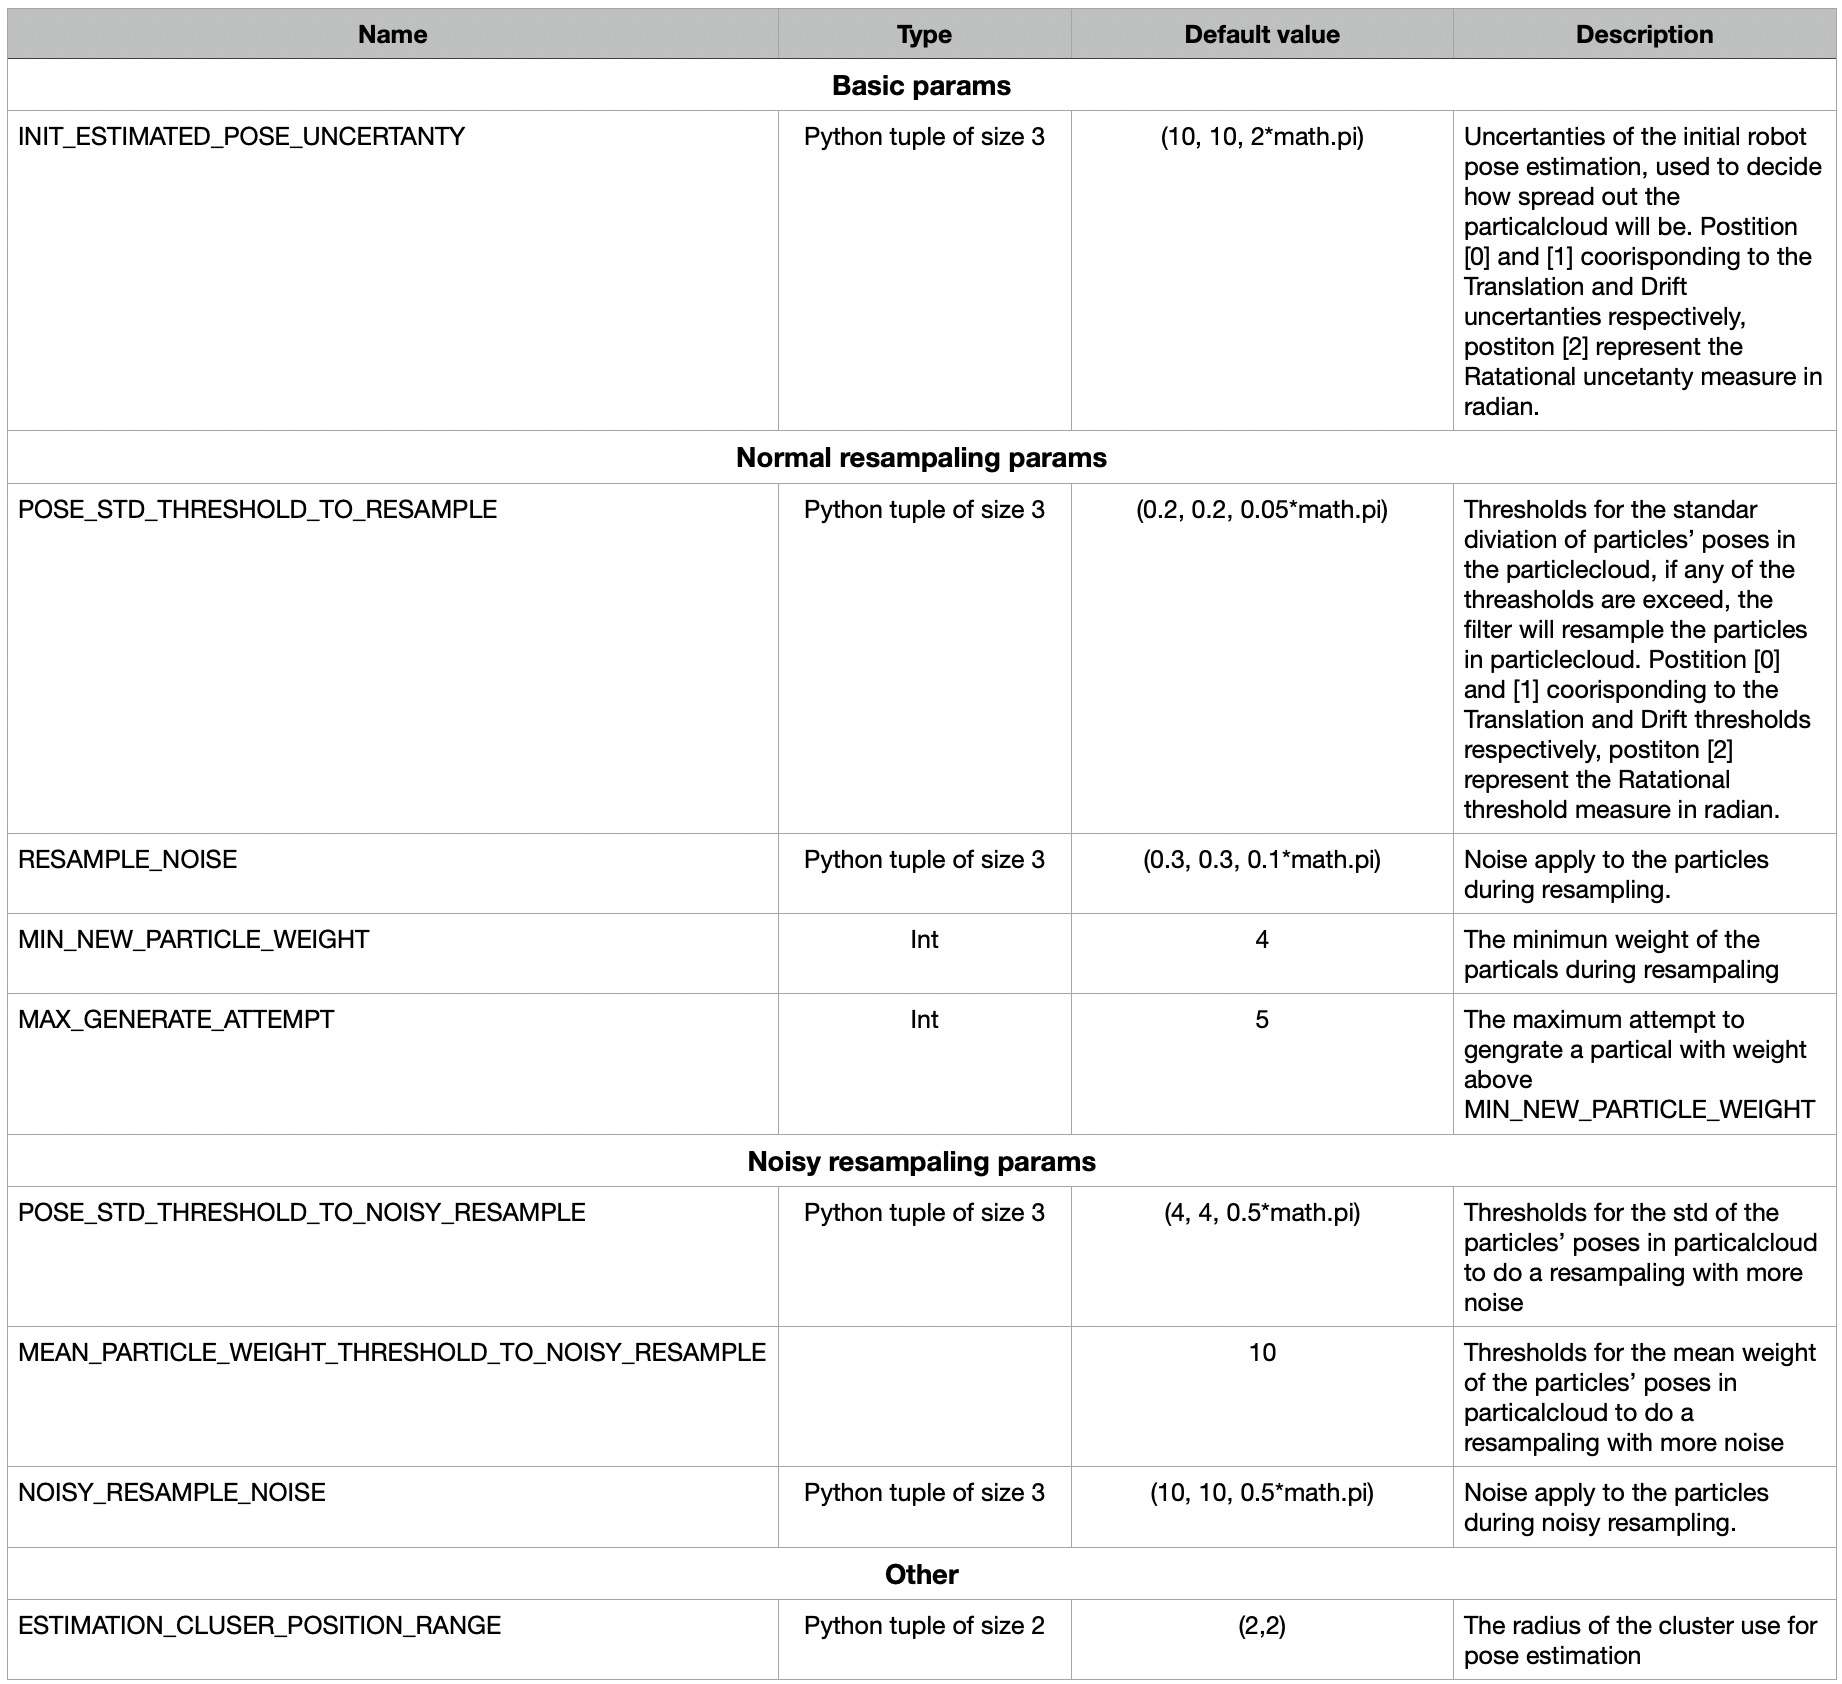
\includegraphics[width=16cm, height=14cm]{Const.png}
      \end{figure}

  % \section{Helper functions}
  %   \subsection{blue\_info\_logging(msg) and yellow\_info\_logging(msg)}
  %     Helper functions, useful for debugging and giving infomation. Both functions take a string as an argument and will 
  %     output highlighted text in the terminal during runtime use ROS logging interface with severity level INFO\cite{ROSlogger}. 
  %     \begin{figure}[h]
  %       \centering
  %       \caption{Example output of blue\_info\_logging}
  %       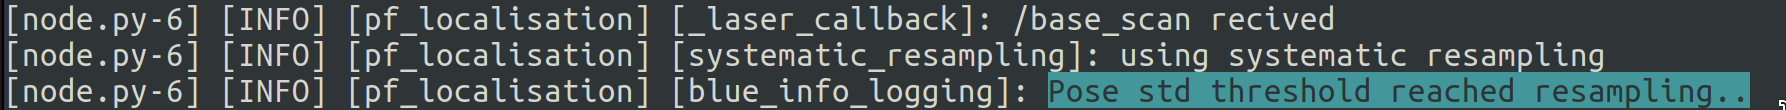
\includegraphics[width=14cm, height=0.9cm]{Blue_logger}
  %       \caption{Example output of yellow\_info\_logging}
  %       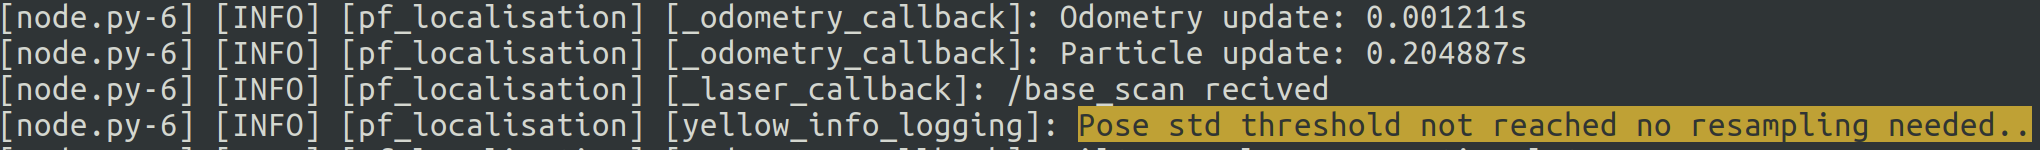
\includegraphics[width=14cm, height=1.1cm]{Yellow_logger}
  %     \end{figure}


  %   \subsection{get\_random\_pose(mean, noise\_range)}
  %     \begin{center}
  %       \begin{tabular}{ |l|l|l| }
  %         \hline
  %       \textbf{Argument} &\textbf{Type} &\textbf{Description} \\ 
  %       \hline
  %       \textit{mean} &Pose & The mean pose that to be apply noise with.\\ 
  %       \hline
  %       \textit{noise\_range} & tuple of size 3 & Tuple discirbe the noise range. Postition [0] and [1]\\
  %       &&coorisponding to the Translation and Drift uncertanties noise,\\
  %       && postiton [2] represent the Ratational noise measure in radian.\\
  %       \hline  
  %       \end{tabular}
  %     \end{center}
  %     Helper function, return a noisy Pose object by adding noise to the mean pose. 
  %     The noisey Position of the return pose are generated randomly following 
  %     gaussian distributions with \textit{mean} as the argument passed into the function and the 
  %     variance is 0.2 * the coorisponding \textit{noise\_range}. The noisey Orintation of the return pose are 
  %     generated by calling the rotateQuaternion() function given, where the radian of the rotation
  %     is also generated randomly with a Gaussian distribution of mean=0, variance=0.2 * \textit{noise\_range[2]}.

  
  %   \subsection{get\_PC\_pose\_std()}
  %   Helper function takes no arguments, will return the standard diviation of the poses in current
  %   \textit{particlecloud} as a tupole of size 3, with postition [0] and [1] coorisponding to the Translation and Drift standard diviations, 
  %   postiton [2] represent the Ratational standard diviation in radian.


  \section{Initialise Particle Cloud}
  The global variable \textit{particlecloud} and \textit{particle\_importance} are initialised in this function.  
  \textit{particlecloud} is initialised by calling the helper function \textit{get\_random\_pose()}, 
  with \textit{initialpose} as the mean and the global constant \textit{INIT\_ESTIMATED\_POSE\_UNCERTANTY} as the noise\_range. 
  This function is repeatly called in a for loop, coltrolled by the global constant \textit{NUMBER\_PREDICTED\_READINGS}, so a cloud of particles 
  are generated around the \textit{initialpose}. \textit{particle\_importance} are initialised to an array of 1s with the size equals to \textit{NUMBER\_PREDICTED\_READINGS}.
  %   the generated poses are append to a PoseArray object, which then return by the function after the for loop. \textit{particle\_importance} are initialised to an array of 1s with the size equals to \textit{NUMBER\_PREDICTED\_READINGS}.
  % \subsection{initialise\_particle\_cloud(initialpose)}
  %   This function will be called when the ROS subscriber recive messages under the topic "\textit{/initialpose}". 
  %   It will assign the globle variables \textit{prev\_odom\_x}, \textit{prev\_odom\_y} and \textit{prev\_odom\_heading} according to the given 
  %   \textit{initialpose}. It is also crucial to set \textit{odom\_initialised} to false, this is because we want to reinitialise the
  %   motion modle between estimations. These globle variables will be used by the motion modle, to move the \textit{particlecloud} and \textit{estimatedpose} accordign 
  %   to the control signal.\\

  %   The global \textit{particlecloud} and \textit{particle\_importance} are also initialised in this function.  \textit{particlecloud} is initialised by calling the helper function \textit{get\_random\_pose()}, with \textit{initialpose} as the mean
  %   and the global variable \textit{INIT\_ESTIMATED\_POSE\_UNCERTANTY} as the noise\_range. This function is repeatly called in a for loop, coltrolled by the global constant \textit{NUMBER\_PREDICTED\_READINGS}.
  %   the generated poses are append to a PoseArray object, which then return by the function after the for loop. \textit{particle\_importance} are initialised to an array of 1s with the size equals to \textit{NUMBER\_PREDICTED\_READINGS}.
    
  \section{Update Particle Cloud}
  In this part, the filter will update the global variable partical\_importance according to the newest scan, 
  and optionally chooes to do a \textit{normal resampaling} of a \textit{noisy resampaling} according to the,
  standard diviation of the poses in particlecloud and the preset constant \textit{POSE\_STD\_THRESHOLD\_TO\_RESAMPLE} 
  and \textit{POSE\_STD\_THRESHOLD\_TO\_NOISY\_RESAMPLE}.
  % This part occours every time when the ROS subscriber \textit{\_laser\_subscriber} recived a \textit{LaserScan} mesage under the topic \textit{/base\_scan}, and the function \textit{update\_particle\_cloud()} will be called\\
  % In the final design of this part, I have decided to not resample the \textit{particlecloud} 
  % every time the function \textit{update\_particle\_cloud()} is called. 
  % The reasons behind this decision is stated in the Design iterations\ref{UPC_DI}.

    % \subsection{update\_particle\_cloud(scan)}
  %     \begin{center}
  %       \begin{tabular}{ |l|l|l| }
  %         \hline
  %       \textbf{Argument} &\textbf{Type} &\textbf{Description} \\ 
  %       \hline
  %       \textit{scan} &sensor\_msgs.msg.LaserScan & The laser scan data of the surrounding environment\\ 
  %       \hline
  %       \end{tabular}
  %     \end{center}
  %     When this function is called, it will first update the global variable \textit{particle\_importance} by calling the \textit{update\_particle\_importance()} helper function with \textit{scan}. 
  %     After this, it will compare the standard diviation of the poses in the particlecloud global variable with the preset constant \textit{POSE\_STD\_THRESHOLD\_TO\_RESAMPLE} to see if 
  %     the standard diviations exceed the thresholds. If this condition is satisfied, then the functuon \textit{systematic\_resampling()} will be called to resample the \textit{particlecloud}.

      \subsection{Update particle importance}
      % \begin{center}
      %   \begin{tabular}{ |l|l|l| }
      %     \hline
      %   \textbf{Argument} &\textbf{Type} &\textbf{Description} \\ 
      %   \hline
      %   \textit{scan} &sensor\_msgs.msg.LaserScan & The laser scan data of the surrounding environment\\ 
      %   \hline
      %   &&\\
      %   \hline
      %   \textbf{\textit{return}} &Numpy Array & The new global \textit{particle\_importance} array \\ 
      %   \hline
      %   \end{tabular}
      % \end{center}
      When this function is called, it will construct an array by iterate throught the poses in \textit{particlecloud} and get its weight by calling the given \textit{get\_weight()} 
      function in sensor model. The elements in the array then averaged with the global \textit{particle\_importance} array's elements. The reason behind this is to previent the accumulated
      weight gets too big and also deal with the situation where the robot is static for a long time but also reciving 
      laser data.

      \subsection{Resampling}
      During this part of the filter, systematic resampaling was used to update the poses in 
      the particlecloud, and noise will be reintroduce to the particles accoring to the preset constances
      \textit{RESAMPLE\_NOISE} or \textit{NOISY\_RESAMPLE\_NOISE}. With one modification to the
      basic systematic resampaling process, I have decided to apply the constrain that the newly
      generated particles cannot below a threshold declare by \textit{MIN\_NEW\_PARTICLE\_WEIGHT},
      this constrain will prevent the particle being generated outside of the map, and will reduced
      the time takes for the particles to converge.
      % \begin{center}
      %   \begin{tabular}{ |l|l|l| }
      %     \hline
      %   \textbf{Argument} &\textbf{Type} &\textbf{Description} \\ 
      %   \hline
      %   \textit{scan} &sensor\_msgs.msg.LaserScan & The laser scan data of the surrounding environment\\ 
      %   \hline
      %   &&\\
      %   \hline
      %   \textbf{\textit{return}} &Pose Array & The new global \textit{particlecloud} \\ 
      %   \hline
      %   &Numpy Array & The new global \textit{particle\_importance} array \\ 
      %   \hline
      %   \end{tabular}
      % \end{center}
      % When this function is called, perform the systematic resampling process for the current \textit{particlecloud}, using the values stored in the \textit{particle\_importance} array
      % and then reintroduce noise to the particles by using the helper function \textit{get\_random\_pose()}, with the current resampaling partical's pose as mean and the preset
      % constant \textit{RESAMPLE\_NOISE} as \textit{noise\_range}.
      
      % I have made a small change to the origional algorithm we have discussed during the lecture, that is not allowing the weight of the newly generated particle to below
      % a threshold, I belive this will help with the speed of convergence and the estimatedpose accuracy.
  \section{Estimate Pose}
  In this part, the filter will first identify the particle with the highest \textit{partical\_importance} value,
  and then return the average pose of the particles around this particle according to the preset
  constant \textit{ESTIMATION\_CLUSER\_POSITION\_RANGE}
  \newpage
  \part{Benchmark}
  \subsection{The kidnapped robot problem}
    \paragraph{}
    The filter was able to deal with some of the kidnapped robot problem, also this is the reason
    why I decided to have 2 different noise for resampaling. It now could work in situation which the movement
    is parallel to the heading of the robot, however have a poor performance, if the movement is perpendicular,
    which i assume is because of the motion modle is not expecting such movement and is not spreading
    the particlecloud perpendicularly.
  \subsection{Simpath1: Estimated position comparered to ground truth}
  \begin{figure}[h]
  \centering
  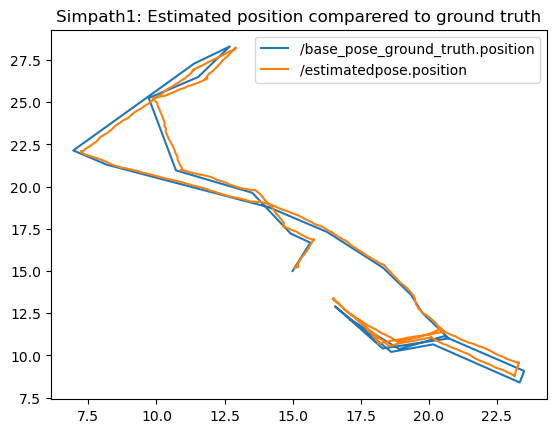
\includegraphics[width=14cm, height=14cm]{sim1_paths.png}
  \end{figure}
  TODO: compare heading
  TODO: calculate RMSE
  \paragraph{}
  The performance of the Particle filter is decent when running the given \textit{Simpath1} bag file,
  the path produced have a roughtly correct shape, most of the diviation happes while the robot is tuning,
  which I tried could be reduced by reducing the preset \textit{POSE\_STD\_THRESHOLD\_TO\_RESAMPLE} constant.
  The bag file used to produce this graph can be found here.
  \newpage
  \subsection{Simpath2: Estimated position comparered to ground truth}
  \begin{figure}[h]
  \centering
  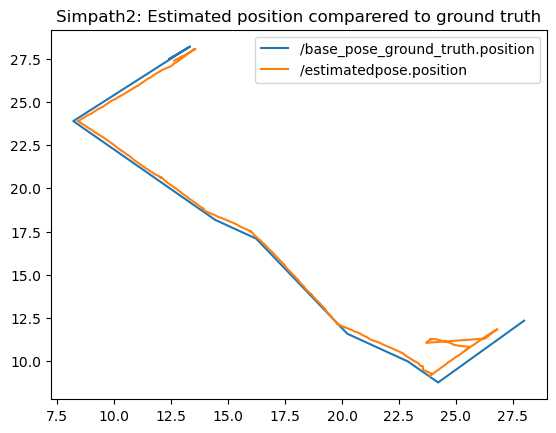
\includegraphics[width=14cm, height=14cm]{sim2_paths.png}
  \end{figure}
  TODO: compare heading
  TODO: calculate RMSE
  \paragraph{}
  The performance of the Particle filter is decent when running the given \textit{Simpath2} bag file,
  However when comparing to the performance on \textit{Simpath1}, it struggled to localise at the start,
  due to the movement of the robot starts sooner also the distance of the movement are further, which left a
  small window for the particles to form a cluster. The bag file used to produce this graph can be found here.
\newpage


\part{Appendix}
\section{Initialise Particle Cloud (Past iterations)}
  \subsection{Iteration\#1 - Random particles according to map size}
  At the start, I had this thinking that if the particles of the filter are more spread out, the particles will
  have a better chance of getting to the correct pose. So I decided to use the dimensions of the map as the variance in an gaussian distribution
  to set the initial noise, so the particles will be very spread out on the map\ref{fig:gbm}. I realised later in the
  delopment process that althought the particles are exploring a lots of places, but the low particle density have led
  to a very slow convergence. Also sometime the actual map might only take up a small space in some of the map files. So 
  I decided using the Map\_info to introduce noise to the particles is not practical.
  \begin{figure}[h]
      \caption{Particlecloud of size 60 generated using map\_info}
      \centering
      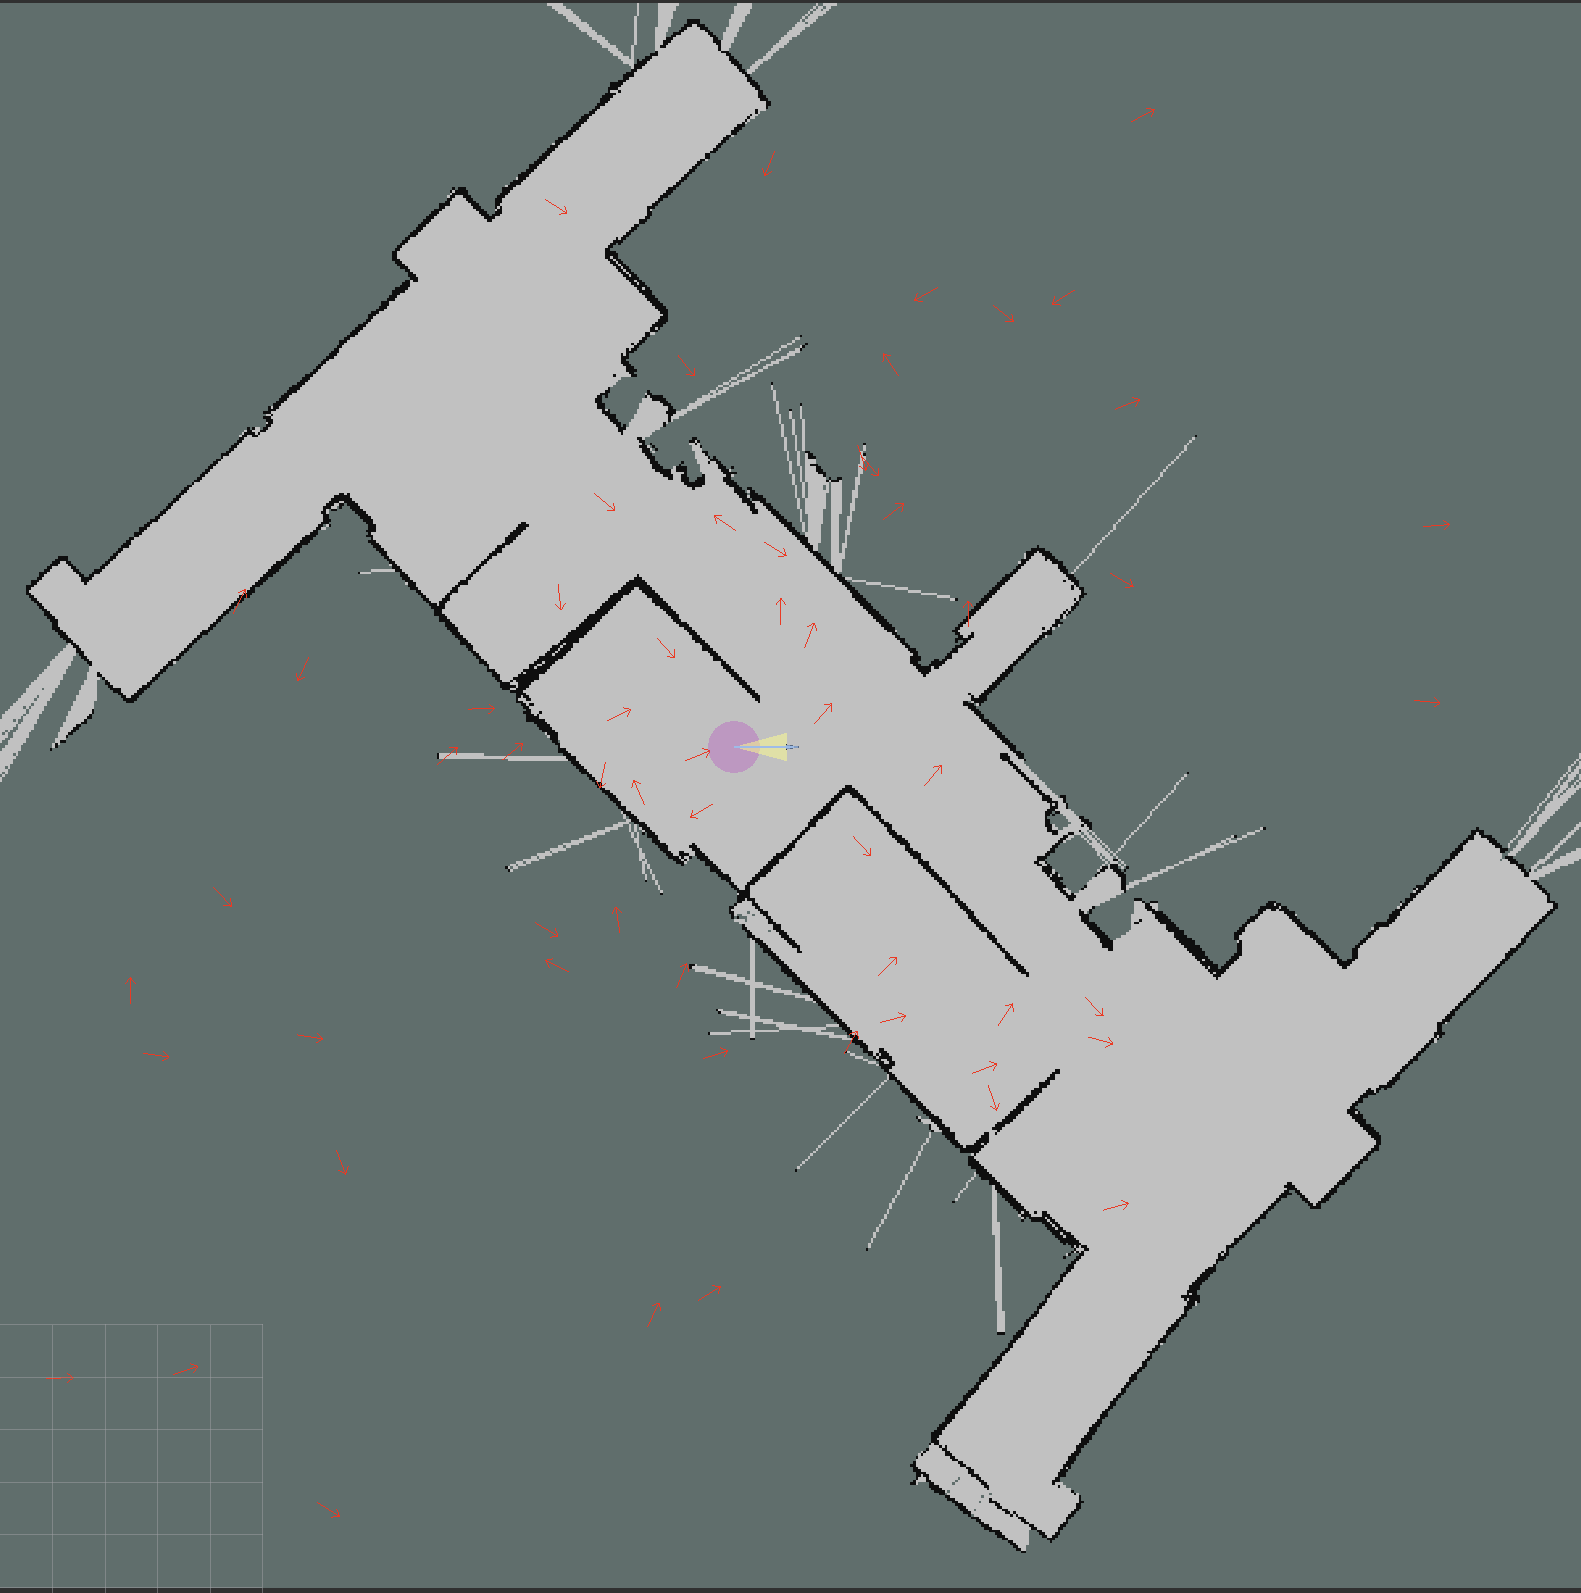
\includegraphics[width=10cm, height=10cm]{gen_by_map_info.png}
      \label{fig:gbm}
    \end{figure}
  \subsection{Iteration\#2 - Random particles according to constants}
    In this iteration, i tried to generate the initial \textit{particlecloud} with constants, which allowed me to
    predict the particle density way better. However hard-coding the constants into the code results in reduced generalisation 
    while runing the filter in different maps. So in my final implementation, I introduced a global constant \textit{INIT\_ESTIMATED\_POSE\_UNCERTANTY},
    which allow user to discribe how inaccurate the initial pose estimation is, and hence control how spread out the particles will be.

\section{Update Particle Cloud (Past iterations)}
\label{UPC_DI}
  \subsection{Iteration\#1 - Resample everytime when laser data is recived}
  This is the iteration where I simply call the \textit{get\_weight()} function in sensor model everytime a base\_scan is recived.
  The problem of doing this is althought the particlecloud will converge into clusters,
  it will result in an very wobbly pose estimation even when the robot is not moving, this is due to the constant updating particlecloud.
  \subsection{Iteration\#2 - Resample according to difference in accumulated particle\_importance}
  After decided I do not want to resample the particlecloud everytime this function is called, I came up with the idea to accumulate the
  weight of the particles before resampaling, thinking that this will favour the more weighted particles because the there will be a bigger
  difference in importance between the more accurate particles and the less accurate ones. The result of this has reduced the frequency of resampaling,
  however it also increased the time taken for the initial convergence of the particlecloud.
  % \subsection{Iteration\#3 - Resample according to the variance of particle\_importance}
\section{Estimate Pose (Past iterations)}
  \subsection{Iteration\#1 - Averaging everything}
  \subsection{Iteration\#2 - Taking the particle with hightest weight}
\end{document}

% LocalWords:  lrrrrrrr ment Macduff Kemnay Ruchill FDS mc th fds
% LocalWords:  Anscombe